
% \begin{remark}
%     Avec la strategy Innermost, pour les modules dont la valeur de retour est booleanne, il suffit de donner des regles pour la reponse positive. Tout cela a l'aide d'un constructor "uniform" et le module "if-then-else". exemple: en remplasant l'expression suivante:
% $$eq\_list\_nat(@ * 1, @ * 2)$$
% par 
% $$if\_then\_else(uniform(eq\_list\_nat(@ * 1, @ * 2)), true, false)$$
% on peut connaitre les cas negatives, en raison des trois regles suivantes et la strategy Innermost:
% \begin{flalign*}
%     1\\
%     \hspace{1cm}
%     &if\_then\_else(true, X, Y)
%     \\
%     &\longrightarrow
%     \\
%     &X\\
%     2\\
%     \hspace{1cm}
%     &if\_then\_else(uniform(B), X, Y)
%     \\
%     &\longrightarrow
%      \\
%      &Y\\
%     3\\
%     \hspace{1cm}
%     &uniform(true)
%     \\
%     &\longrightarrow
%     \\
%     &true
% \end{flalign*}
% Pour appliquer la deuxieme regle, il faut que B soit en forme normal, sinon $uniform(B)$ n'est pas en forme normal. De plus, il faut que $B \not \equiv true$, sinon $uniform(B)$ peut etre reduit en $true$ par la troisieme regle.
% \begin{itemize}
%     \item on simplifie au fond le module servant a comparer les entiers naturels
%     \item moins de regles: grâce à la statégie innermost et les trois regles mentionnes
%     \item moins de pairs de dependences générés: parcequ'il y a moins de règle
% \end{itemize}

% \end{remark} 

% \begin{remark}
%     Using the Innermost strategy, for modules with boolean return values, it is sufficient to define rules for the positive outcome only. This can be achieved by utilizing a "uniform" constructor and the "if-then-else" module. For example, by replacing the expression:
%     $$eq\_list\_nat(@ * 1, @ * 2)$$
%     with 
%     $$if\_then\_else(uniform(eq\_list\_nat(@ * 1, @ * 2)), true, false),$$
%     negative cases can be handled due to the following three rules and the Innermost strategy:
%     \begin{flalign*}
%         1. &\hspace{1cm} if\_then\_else(true, X, Y) \longrightarrow X \\
%         2. &\hspace{1cm} if\_then\_else(uniform(B), X, Y) \longrightarrow Y \\
%         3. &\hspace{1cm} uniform(true) \longrightarrow true
%     \end{flalign*}
%     To apply the second rule, $B$ must be in normal form; otherwise, $uniform(B)$ will not be in normal form. Additionally, $B$ must not be equivalent to $true$, as $uniform(B)$ could be reduced to $true$ by the third rule.


%     % \begin{itemize}
%     %     \item Simplifies the module used for comparing natural numbers.
%     %     \item Fewer rules are required, thanks to the Innermost strategy and the three mentioned rules.
%     %     \item Fewer dependency pairs are generated due to the reduced number of rules.
%     % \end{itemize}
% \end{remark}
This section designs a hierarchical term rewriting system (HTRS) to simulate graph relabeling systems. It introduces two sets of modules: one specific to each graph relabeling system and the other common to all. These modules manage tasks such as generating and comparing graphs, checking for forbidden contexts, identifying applicable rewriting rules, and applying rewriting steps.

\begin{example}
    \label{example_fcpgrs}
    We present our translation using the graph relabeling system with priorities and forbidden contexts, $\mathcal{R} \mathop{=} \{r_1,\ r_2,\ r_3\}$
  
    \begin{tikzpicture}
      \draw (-1,0) node[left] {$r_1$:};
      \draw (1,0) node[above] {0};
      
      \node[draw,circle] (x_1) at (0,0) {$1$};
      \draw (0,0.3) node[above]{A};
      \node[draw,circle, minimum size \mathop{=} 1pt] (x_2) at (2,0) {$2$};
      \draw (2,0.3) node[above]{N};
      \draw[-] (x_1) -- (x_2);
      
      \draw (3,0) node[right] {$\longrightarrow$};
      \draw (6,0) node[above] {1};
      
      \node[draw,circle] (x3) at (5,0) {$1$};
      \draw (5,0.3) node[above]{A};
      \node[draw,circle, minimum size \mathop{=} 1pt] (x4) at (7,0) {$2$};
      \draw (7,0.3) node[above]{A'};
      \draw (7.5,-0.45) node[above]{$,$};
      \draw (8,-0.45) node[above]{$\Big\{$};
  
      % Context 2
      \node[draw,circle](c2_1) at (11,0.75) {$1$};
      \draw (11,1) node[above] {N};
      \draw (10.25,-1) node[below] {A};
      \draw (11.75,-1) node[below] {A'};
      \node[draw,circle](c2_2) at (10.25,-0.75) {$2$};
      \node[draw,circle](c2_3) at (11.75,-0.75) {$3$};
      \draw[-] (c2_1) -- (c2_2);
      \draw (10.6,0) node[left] {0};
      \draw (11.35,0) node[right] {0};
      \draw[-] (c2_1) -- (c2_3);
  
      \draw (12.5,-0.45) node[above]{$\Big\}$};
      \draw[-] (x3) -- (x4);
    \end{tikzpicture}
    
    \begin{tikzpicture}
      \draw (-1,0) node[left] {$r_2$:};
      \draw (1,0) node[above] {0};
      
      \node[draw,circle] (x_1) at (0,0) {$1$};
      \draw (0,0.3) node[above]{A'};
      \node[draw,circle, minimum size \mathop{=} 1pt] (x_2) at (2,0) {$2$};
      \draw (2,0.3) node[above]{N};
      \draw[-] (x_1) -- (x_2);
      
      \draw (3,0) node[right] {$\longrightarrow$};
      \draw (6,0) node[above] {1};
      
      \node[draw,circle] (x3) at (5,0) {$1$};
      \draw (5,0.3) node[above]{A'};
      \node[draw,circle, minimum size \mathop{=} 1pt] (x4) at (7,0) {$2$};
      \draw (7,0.3) node[above]{A'};
      \draw (7.5,-0.45) node[above]{$,$};
      \draw (8,-0.45) node[above]{$\Big\{$};
      \draw (8.5,-0.45) node[above]{$\Big\}$};
      \draw[-] (x3) -- (x4);
    \end{tikzpicture}
    
    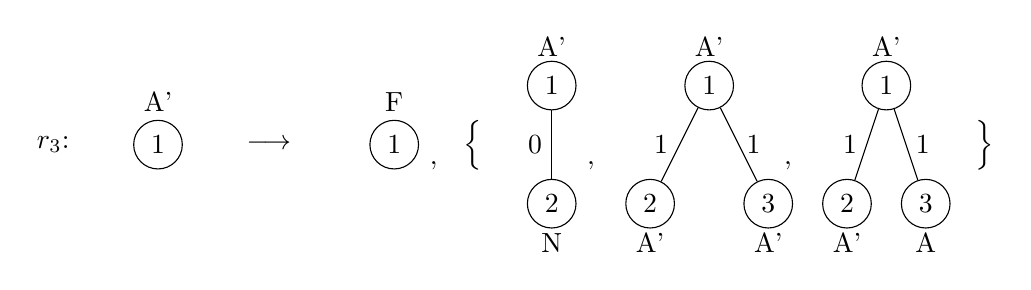
\begin{tikzpicture}
      \draw (-1,0) node[left] {$r_3$:};
      
      \node[draw,circle] (x_1) at (0,0) {$1$};
      \draw (0,0.3) node[above]{A'};
      
      \draw (1,0) node[right] {$\longrightarrow$};
      
      \node[draw,circle] (x3) at (3,0) {$1$};
      \draw (3,0.3) node[above]{F};
      
      % Context 1
      \node[draw,circle](c1_1) at (5,0.75) {$1$};
      \draw (5,1) node[above] {A'};
      \node[draw,circle](c1_2) at (5,-0.75) {$2$};
      \draw (5,-1) node[below] {N};
      \draw (5,0) node[left] {0};
      \draw[-] (c1_1) -- (c1_2);
      \draw (5.5,-0.45) node[above]{$,$};
      
      % Context 2
      \node[draw,circle](c2_1) at (7,0.75) {$1$};
      \draw (7,1) node[above] {A'};
      \draw (6.25,-1) node[below] {A'};
      \draw (7.75,-1) node[below] {A'};
      \node[draw,circle](c2_2) at (6.25,-0.75) {$2$};
      \node[draw,circle](c2_3) at (7.75,-0.75) {$3$};
      \draw[-] (c2_1) -- (c2_2);
      \draw (6.6,0) node[left] {1};
      \draw (7.35,0) node[right] {1};
      \draw[-] (c2_1) -- (c2_3);
      \draw (8,-0.45) node[above]{$,$};
      
      % Context 3
      \node[draw,circle](c3_1) at (9.25, 0.75) {$1$};
      \node[draw,circle](c3_2) at (8.75, -0.75) {$2$};
      \node[draw,circle](c3_3) at (9.75, -0.75) {$3$};
      \draw (9.25,1) node[above] {A'};
      \draw (8.75,-1) node[below] {A'};
      \draw (9.75,-1) node[below] {A};
      \draw (9,0) node[left] {1};
      \draw (9.5,0) node[right] {1};
      \draw[-] (c3_1) -- (c3_2);
      \draw[-] (c3_1) -- (c3_3);
      
      \draw (3.5,-0.45) node[above]{$,$};
      \draw (4,-0.45) node[above]{$\Big\{$};
      \draw (10.5,-0.45) node[above]{$\Big\}$};
    \end{tikzpicture}
  \end{example} 
  




  \subsection{System-Specific Modules}


%   \subsection*{get\_context\_rule\_graphs}
%     \begin{flalign*}
%         \hspace{1cm}
%         1. \\
%         &get\_context\_rule\_graphs(n) &\\
%         &\longrightarrow &\\
%         &\overline{rule\_and\_context\_graphs(n)} &
%     \end{flalign*}

%     Given a rule number $n$, $get\_context\_rule\_graphs(n)$ returns the concatenantion of terms $graph(r,c,k)$ for all $c \mathop{\in}  where $r$ is the rule number, $c$ is the context number (0 for the rule graph), and $K$ is the size of the graph. Subterms are ordered according to the topological order of the priority.

\subsection*{get\_context\_rule\_graphs}
\begin{flalign*}
    \hspace{1cm}
    &get\_context\_rule\_graphs(R) &\\
    &\longrightarrow &\\
    &\circledast \{graph(R, c, k) \mathop{\mid} 0 \leq c \leq \operatorname{length}(f(r_R))
    %  \mathop{\land} (c \mathop{=} 0 \implies k \mathop{=} |lhs(r_N)|) \mathop{\land} 
    % (c \mathop{\geq} 1 \implies k \mathop{=} |\operatorname{codom}(f(r_N))|)
    \} &
\end{flalign*}

where $N$ is the rule number. The right-hand side (rhs) is the concatenation of terms in $\{ graph(R, c, k) \mathop{\mid} 0 \leq c \leq \operatorname{length}(f(r_N))\}$. If $c \mathop{=} 0$, then $k$ is the size of the left-hand side (lhs) graph of the $N$-th rule. Otherwise, $c \mathop{\geq} 1$ and $k$ is the size of the domain of the $c$-th forbidden context of the $N$-th rule.
    

    \subsection*{generate\_graph}
  
\begin{flalign*}
    \hspace{1cm}
    &generate\_graph(R, C, @ * X_n * X_{n-1} * \ldots * X_2 * X_1) & \\
    &\longrightarrow & \\
    & \lambda(node(x_1), l_{node(x_1)}) * \ldots * \lambda(node(x_n), l_{node(x_n)}) * & \\
    & \lambda(edge(x_1,x_2), l_{edge(x_1,x_2)}) * \lambda(edge(x_1,x_3), l_{edge(x_1,x_3)}) * \ldots * \lambda(edge(x_1,x_n), l_{edge(x_1,x_n)}) * & \\
    & \lambda(edge(x_2,x_1), l_{edge(x_2,x_1)}) * \lambda(edge(x_2,x_3), l_{edge(x_2,x_3)}) * \ldots * \lambda(edge(x_2,x_n), l_{edge(x_2,x_n)}) * & \\
    & \ldots & \\
    & \lambda(edge(x_n,x_1), l_{edge(x_n,x_1)}) * \lambda(edge(x_n,x_2), l_{edge(x_n,x_2)}) * \ldots * \lambda(edge(x_n,x_{n-1}), l_{edge(x_n,x_{n-1})}) &
\end{flalign*}
where $R$ is the rule number,  $C$ the number of graph in the rule $r_R$, $n$ the size of the lhs graph, if $C=0$, of the rule $r_R$ or the size of the codomain of the $C$-th of the rule. The context or lhs rule graph; subterms are ordered. The rhs of this rule is the representation of the corresponding labeled graph.

\subsection*{occurrence\_to\_rewrite\_step}

\noindent For each rule $R$ in the FC-P-GRS, there is a corresponding specific rule:
\begin{flalign*}
    \hspace{1cm}
    &occurrence\_to\_rewrite\_step(N, X) & \\
    &\longrightarrow & \\
    &\Gamma(\tau(rhs(r_N)), X)
\end{flalign*}
where $N$ is the rule numnber, $X$ is a term encoding all nodes participating to the rewriting step, and $\Gamma(\tau(rhs(r_N)), X)$ is the representation of the right-hand side of rule $r_N$ but every number $k$ is replaced by $X_k$.

    
    
    \subsection*{main}
    Combining with the innermost strategy, this module allows us to simply our translation by focusing only in the case where $s$ can be reduced to true for every $uniform(s)$.  
    \begin{flalign*}
        & main(
        \\ & \hspace{1cm} LabellingFunction, 
        \\ & \hspace{1cm} @
        \\ & \hspace{1cm} \vdots
        \\ & \hspace{1cm} @
        \\ & )
        \\
        &\longrightarrow
        \\
        & main(
            \\ & \hspace{1cm} LabellingFunction, 
            \\ & \hspace{1cm} identify\_applicable\_occs\_of\_rule(
                \\ & \hspace{2cm} LabellingFunction,
                \\ & \hspace{2cm} get\_context\_rule\_graphs(1), 
                \\ & \hspace{2cm} @, 
                \\ & \hspace{2cm} @,
            \\ & \hspace{1cm}),
            \\ & \hspace{1cm} identify\_applicable\_occs\_of\_rule(
                \\ & \hspace{2cm} LabellingFunction,
                \\ & \hspace{2cm} get\_context\_rule\_graphs(2), 
                \\ & \hspace{2cm} @, 
                \\ & \hspace{2cm} @,
            \\ & \hspace{1cm}),
            \\ & \hspace{1cm} \vdots
            \\ & \hspace{1cm} identify\_applicable\_occs\_of\_rule(
                \\ & \hspace{2cm} LabellingFunction,
                \\ & \hspace{2cm} get\_context\_rule\_graphs(n), 
                \\ & \hspace{2cm} @, 
                \\ & \hspace{2cm} @,
            \\ & \hspace{1cm}),
            \\ & )
    \end{flalign*} \\

    \begin{flalign*}
        & main(
            \\ & \hspace{1cm} LabellingFunction, 
            \\ & \hspace{1cm} identify\_applicable\_occs\_of\_rule(
                \\ & \hspace{2cm} X_1
                \\ & \hspace{2cm} X_2        
                \\ & \hspace{2cm} X_3
                \\ & \hspace{2cm} X_4
            \\ & \hspace{1cm}),
            \\ & \hspace{1cm} identify\_applicable\_occs\_of\_rule(
                \\ & \hspace{2cm} X_5
                \\ & \hspace{2cm} X_6
                \\ & \hspace{2cm} X_7 
                \\ & \hspace{2cm} X_8
            \\ & \hspace{1cm}),
            \\ & \hspace{1cm} \vdots
            \\ & \hspace{1cm} identify\_applicable\_occs\_of\_rule(
                \\ & \hspace{2cm} X_{4n-3}
                \\ & \hspace{2cm} X_{4n-2}
                \\ & \hspace{2cm} X_{4n-1}
                \\ & \hspace{2cm} X_{4n}
            \\ & \hspace{1cm}),
            \\ & )
        \\
        &\longrightarrow
        \\
        & LabellingFunction
    \end{flalign*} \\

    \begin{flalign*}
        1 \le k \le n
        \\ 
        & main(
        \\ & \hspace{1cm} LabellingFunction, 
        \\ & \hspace{1cm} X_1
        \\ & \hspace{1cm} X_2
        \\ & \hspace{1cm} \vdots
        \\ & \hspace{1cm} X_{k-1}
        \\ & \hspace{1cm} some(X_k)
        \\ & \hspace{1cm} X_{k-1}
        \\ & \hspace{1cm} \vdots
        \\ & \hspace{1cm} X_n
        \\ & )
        \\
        &\longrightarrow
        \\
        & main(
        \\ & \hspace{1cm} rewrite(
            \\ & \hspace{2cm} LabellingFunction,
            \\ & \hspace{2cm} generate\_occurrence\_to\_rewrite\_step(k, X_k)
        \\ & \hspace{1cm}) 
        \\ & \hspace{1cm} @
        \\ & \hspace{1cm} \vdots
        \\ & \hspace{1cm} @
        \\ & )
    \end{flalign*} \\


    \subsection*{Wrap}
    With this module and the innermost strategy, we can distinguish boolean expressions that can be evaluated to "true" and others.    

    \begin{flalign*}
        \\ & uniform(true) \longrightarrow true
    \end{flalign*}

    
    \subsection{General Modules}

    The following terminating modules are common for every FCGLS translation.

    \subsection*{if\_then\_else}

    \begin{flalign*}
        \hspace{1cm}
        &if\_then\_else(true, X, Y)&
        \\
        &\longrightarrow
        \\
        &X\\
        \hspace{1cm}
        &if\_then\_else(uniform(B), X, Y)&
        \\
        &\longrightarrow
         \\
         &Y
    \end{flalign*}


    \subsection*{eq\_list\_nat} 
    This module tests if two arguments encode the same list of natural numbers.

    \begin{flalign*}
        &eq\_list\_nat(X * Z, Y * Z)
        \\
        &\longrightarrow
        \\
        &eq\_list\_nat(X, Y)
        \\
        \hspace{1cm}
        &eq\_list\_nat(@, @)
        \\
        &\longrightarrow
        \\
        &true
    \end{flalign*}

    \subsection*{eq\_noe }
    This module compares two terms encoding nodes (or edges) and returns true if they encode the same node (or edge).

    \begin{flalign*}
        \hspace{1cm}
        & eq \_noe(node(X), node(X)) &
        \\
        & \longrightarrow
        \\
        & true
    \end{flalign*}
    
    % \begin{flalign*}
    %     4\\
    %     \hspace{1cm}
    %     & eq \_noe(edge( X, Y), edge( Z, W)) &\\
    %     & \longrightarrow\\
    %     & et(
    %        \\ & \hspace{1cm}eq\_nat(X, Z),
    %        \\ & \hspace{1cm}eq\_nat(Y,W)
    %     \\ & )
    % \end{flalign*}
    \begin{flalign*}
        & eq \_noe(edge( X, Y), edge( X, Y)) &\\
        & \longrightarrow\\
        & true
    \end{flalign*}

    \subsection*{mem} 
    This module tests if the first argument is an element of the second argument.

    \begin{flalign*}
        \hspace{1cm}
        &mem(X, Y * Z) & 
        \\
        &\longrightarrow
        \\
        &if\_then\_else(
            \\ & \hspace{1cm} uniform(eq\_list\_nat(@ * X, @ * Z)),
            \\ & \hspace{1cm} true,
            \\ & \hspace{1cm} mem(X, Y)
        \\ & )
    \end{flalign*}

    \subsection*{union}
    This module returns the concatenation of two lists.

    \begin{flalign*}
        \hspace{1cm}
        &union(L_1 * X, L_2)&
        \\
        &\longrightarrow
        \\
        &union(L_1, L_2 * X)&
        \\
        \\
        &union(@, L)&
        \\
        &\longrightarrow
        \\
        &L&
    \end{flalign*}

    
    % \subsection*{cons\_n}
    % cons\_n(x,l) locates the n-th list of $l_1$ and then adds x in the list :
    % \begin{flalign*}
    %     1\\
    %     \hspace{1cm}
    %     &cons \_n(
    %         \\ & \hspace{1cm} s(s(N)),
    %         \\ & \hspace{1cm} X,
    %         \\ & \hspace{1cm} L * Y
    %         \\ &)&
    %     \\
    %     &\longrightarrow
    %     \\
    %     &cons \_n(
    %         \\ & \hspace{1cm} s(N),
    %         \\ & \hspace{1cm} X,
    %         \\ & \hspace{1cm} L
    %         \\ &) * Y 
    % \end{flalign*}
    % Insert :   
    % \begin{flalign*}
    %     2\\
    %     \hspace{1cm}
    %     &cons \_n(s(o), X, L * Y)&
    %     \\
    %     &\longrightarrow
    %     \\
    %     &L * (Y * X)
    % \end{flalign*} 

    
    
    \subsection*{prefix}
    \noindent \texttt{prefix(X, Y) \mathop{=} true} if and only if the list \texttt{Y} is a prefix of the list \texttt{X}.
    
    
    \begin{flalign*}
        \hspace{1cm}
        &prefix(X, @) &
        \\
        &\longrightarrow 
        \\
        &true&
    \end{flalign*}
    % \begin{flalign*}
    %     \hspace{1cm}
    %     2\\
    %     &prefix(X * Y, W * Z)&
    %     \\
    %     &\longrightarrow 
    %     \\
    %     &and(
    %         \\ & \hspace{1cm} eq\_nat(Y,Z),
    %         \\ & \hspace{1cm} prefix(X, W),
    %         \\ &)
    % \end{flalign*}
    \begin{flalign*}
        \hspace{1cm}
        &prefix(X * Z, Y * Z)&
        \\
        &\longrightarrow 
        \\ &prefix(X, Y),
    \end{flalign*}



    \subsection*{graph\_to\_list\_nat}
    Given a graph labeling function encoded by $@ * \lambda(x_1,l_1) * \ldots * \lambda(x_n,l_n)$, this module returns the list $@ * l_1 * \ldots * l_n$.

    \begin{flalign*}
        \hspace{1cm}
        & graph\_to\_list\_nat(X * \lambda(Y,Z))&
        \\
        &\longrightarrow
        \\
        & graph\_to\_list\_nat(X) * Z
        \\
        \\
        & graph\_to\_list\_nat(@)&
        \\
        &\longrightarrow
        \\
        & @
    \end{flalign*}
    
    \subsection*{find\_label}
    This constructor's first argument is a node or an edge of a graph, and the second argument encodes the labeling function of the graph. It returns the label of the first argument.

        \begin{flalign*}
        \hspace{1cm}
        &find\_label(
            \\ & \hspace{1cm} X,
            \\ & \hspace{1cm} F\ *\ \lambda(Y, L)
            \\ &)
        \\
        &\longrightarrow
        \\
        &if\_then\_else(
            \\ & \hspace{1cm} uniform(eq\_noe(X,Y)),
            \\ & \hspace{1cm} L,   
            \\ & \hspace{1cm} find\_label(X, F)
            \\ &)
    \end{flalign*}
    % \noindent According to the result of key-comparison, either we return the label found or continue our recherche:
    % \begin{flalign*}
    %     2\\ 
    %     \hspace{1cm}
    %     &find\_label(X, F\ *\ \lambda(Y, L),true)&
    %     \\
    %     &\longrightarrow
    %     \\
    %     &L &
    % \end{flalign*}

    
    \subsection*{rewrite\_noe}
    Given a labeling function of a graph as the first argument and a node or an edge $K_2$ with label $L_2$ of the graph as the third argument, this module relabels the node or the edge.
    \begin{flalign*}
        \hspace{1cm}
        &rewrite\_noe(
            \\ & \hspace{1cm} F_1 * \lambda(K_1, L_1), 
            \\ & \hspace{1cm} F_2,
            \\ & \hspace{1cm} \lambda(K_2, L_2)
            \\ &)
        \\
        &\longrightarrow
        \\
        &if\_then\_else(
            \\ & \hspace{1cm} uniform(eq\_noe(K_1,K_2)),
            \\ & \hspace{1cm} union(F_1 * \lambda(K_1, L_2),F_2 ),
            \\ & \hspace{1cm} rewrite\_noe(
                \\ & \hspace{2cm} F_1,
                \\ & \hspace{2cm} F_2 * \lambda(K_1, L_1),
                \\ & \hspace{2cm} \lambda(K_2, L_2)
            \\ & \hspace{1cm})
            \\ & )
    \end{flalign*}
    
    % \begin{flalign*}
    %     2\\
    %     \hspace{1cm}
    %     &rewrite\_noe(
    %         \\ & \hspace{1cm} F_1 * \lambda(K_1, L_1), 
    %         \\ & \hspace{1cm} F_2,
    %         \\ & \hspace{1cm} \lambda(K_2, L_2)
    %         \\ &)
    %     \\
    %     &\longrightarrow
    %     \\
    %     &if\_then\_else(
    %         \\ & \hspace{1cm} eq\_noe(K_1,K_2),
    %         \\ & \hspace{1cm}rewrite\_noe(
    %             \\ & \hspace{2cm} F_1 * \lambda(K_1, L_2), 
    %             \\ & \hspace{2cm} F_2,
    %             \\ & \hspace{2cm} @
    %             \\ & \hspace{1cm}),
    %         \\ & \hspace{1cm} rewrite\_noe(
    %             \\ & \hspace{2cm} F_1,
    %             \\ & \hspace{2cm} F_2 * \lambda(K_1, L_1),
    %             \\ & \hspace{2cm} \lambda(K_2, L_2)
    %         \\ & \hspace{1cm})
    %         \\ & )
    % \end{flalign*}

    % \begin{flalign*}
    %     3\\
    %     \hspace{1cm}
    %     &rewrite\_noe(
    %         \\ & \hspace{1cm} F_1, 
    %         \\ & \hspace{1cm} F_2 * X,
    %         \\ & \hspace{1cm} @
    %         \\ &)
    %     \\
    %     &\longrightarrow
    %     \\
    %     &rewrite\_noe(
    %         \\ & \hspace{1cm} F_1 * X, 
    %         \\ & \hspace{1cm} F_2,
    %         \\ & \hspace{1cm} @
    %         \\ &)
    % \end{flalign*}

    % \begin{flalign*}
    %     4\\
    %     \hspace{1cm}
    %     &rewrite\_noe(
    %         \\ & \hspace{1cm} F_1, 
    %         \\ & \hspace{1cm} @,
    %         \\ & \hspace{1cm} @
    %         \\ &)
    %     \\
    %     &\longrightarrow
    %     \\
    %     &F_1
    % \end{flalign*}


    \subsection*{rewrite}
    Given a labeling function of a graph and a labeling function of a subgraph of the graph, this module relabels nodes and edges in the graph according to the subgraph labeling function.

    \begin{flalign*} 
        \hspace{1cm}
        \\ &rewrite(
            \\ & \hspace{1cm} F_1,
            \\ & \hspace{1cm} F_2 * X
            \\ &)&
        \\
        &\longrightarrow
        \\
        &rewrite(
            \\ & \hspace{1cm} rewrite\_noe(
                \\ & \hspace{2cm} F_1,
                \\ & \hspace{2cm} @,
                \\ & \hspace{2cm} X
                \\ & \hspace{1cm}),
            \\ & \hspace{1cm} F_2
        \\ &)
    \end{flalign*}
    \begin{flalign*}
        \hspace{1cm}
        \\ &rewrite(
            \\ & \hspace{1cm} F,
            \\ & \hspace{1cm} @
        \\ &)
        \\
        &\longrightarrow
        \\
        &F
    \end{flalign*}
    
    
    % \subsection*{apply\_rewrite\_steps}

    % \begin{flalign*}
    %     \hspace{1cm}
    %     1\\
    %     &apply\_rewrite\_steps(
    %         \\ & \hspace{1cm} X * Y,
    %         \\ & \hspace{1cm} F
    %     \\ & )
    %     \\
    %     &\longrightarrow
    %     \\
    %     &apply\_rewrite\_steps(
    %         \\ & \hspace{1cm} X,
    %         \\ & \hspace{1cm} rewrite(F, Y)
    %     \\ & )	
    % \end{flalign*}

    % \begin{flalign*}
    %     \hspace{1cm}
    %     2\\
    %     &apply\_rewrite\_steps(
    %         \\ & \hspace{1cm} @,
    %         \\ & \hspace{1cm} F
    %     \\ & )
    %     \\
    %     &\longrightarrow
    %     \\
    %     &F&
    % \end{flalign*}
    
    
    \subsection*{context\_inclusion\_check}
    This module is designed to make the translation easier to understand.
    \begin{flalign*}
        \hspace{1cm}
        1\\
        & context\_inclusion\_check( R, C)&
        \\
        &\longrightarrow
        \\
        & prefix(R, C)
    \end{flalign*}
    
    
    \subsection*{generate\_complete\_graph}
    Let $x_1,\ldots,x_n$ be natural numbers, $generate\_complete\_graph(@ * x_n * \ldots * x_1,\ @ * x_n * \ldots * x_1,\ @ * x_n * \ldots * x_1,\ @ * x_n * \ldots * x_1,\ @)$
       returns the following term encoding the unlabeled complete graph below:
        \begin{align*}
            & node(x_1) * \ldots * node(x_n) * \\
            & edge(x_1,x_2) * edge(x_1,x_3) * \ldots * edge(x_1,x_n) * \\
            & edge(x_2,x_1) * edge(x_2,x_3) * \ldots * edge(x_2,x_n) * \\
            & \ldots \\
            & edge(x_n,x_1) * edge(x_n,x_2) * \ldots * edge(x_n,x_{n-1})
        \end{align*}
    
    \begin{flalign*}
        1\\
        \hspace{1cm}
        &generate\_complete\_graph(
            \\ & \hspace{1cm} L_1,
            \\ & \hspace{1cm} L_2,
            \\ & \hspace{1cm} L_3, 
            \\ & \hspace{1cm} L_4 * X,
            \\ & \hspace{1cm} L_5
        \\ &)
        \\
        &\longrightarrow
        \\
        &generate\_complete\_graph(
            \\ & \hspace{1cm} L_1,
            \\ & \hspace{1cm} L_2,
            \\ & \hspace{1cm} L_3, 
            \\ & \hspace{1cm} L_4,
            \\ & \hspace{1cm} L_5 * node(X)
        \\ & )
    \end{flalign*}
    \begin{flalign*}
        2\\
        &generate\_complete\_graph(
            \\ & \hspace{1cm} L_1,
            \\ & \hspace{1cm} L_2 * X,
            \\ & \hspace{1cm} L_3 * Y,
            \\ & \hspace{1cm} @,
            \\ & \hspace{1cm} L_4
        \\ &)
        \\
        &\longrightarrow
        \\
        &if\_then\_else(
            \\ & \hspace{1cm} uniform(eq\_list\_nat(@ * X, @ * Y)), 
            \\ & \hspace{1cm} generate\_complete\_graph(
                \\ & \hspace{2cm} L_1,
                \\ & \hspace{2cm} L_2 * X, 
                \\ & \hspace{2cm} L_3,
                \\ & \hspace{2cm} @,
                \\ & \hspace{2cm} L_4
            \\ & \hspace{1cm}),
            \\ & \hspace{1cm} generate\_complete\_graph(
                \\ & \hspace{2cm} L_1,
                \\ & \hspace{2cm} L_2 * X, 
                \\ & \hspace{2cm} L_3,
                \\ & \hspace{2cm} @,
                \\ & \hspace{2cm} L_4 * edge(X,Y)
            \\ & \hspace{1cm})
        \\ &)
    \end{flalign*}
    \begin{flalign*}
        3\\
        &generate\_complete\_graph(
            \\ & \hspace{1cm} L_1, 
            \\ & \hspace{1cm} L_2 * X, 
            \\ & \hspace{1cm} @, 
            \\ & \hspace{1cm} @,
            \\ & \hspace{1cm} L3
        \\ &)
        \\
        &\longrightarrow 
        \\
        &generate\_complete\_graph(
            \\ & \hspace{1cm} L_1,   
            \\ & \hspace{1cm} L_2,
            \\ & \hspace{1cm} L_1,
            \\ & \hspace{1cm} @,
            \\ & \hspace{1cm} L3
        \\ & )
    \end{flalign*}
    \begin{flalign*}
        4\\
        &generate\_complete\_graph(
            \\ & \hspace{1cm} L_1, 
            \\ & \hspace{1cm} @, 
            \\ & \hspace{1cm} L_2, 
            \\ & \hspace{1cm} @, 
            \\ & \hspace{1cm} L_3
        \\ &)&
        \\
        &\longrightarrow
        \\
        &L_3&
    \end{flalign*}
    
    
    \subsection*{construct\_induced\_graph}
    Given a labeling function of a graph $F$ and a list $X$ of nodes in the graph, $generate\_complete\_graph(X,@,F)$ return the subgraph induced by nodes in $X$.  
    % \begin{description}
    %     \item[input] $@ * x_n * x_{n-1} * \ldots * x_1$
    %     \item[output]
    %     \begin{align*}
    %         & \lambda(node(x_1), l_{node(x_1)}) * \ldots * \lambda(node(x_n), l_{node(x_n)}) * \\
    %         & \lambda(edge(x_1,x_2), l_{edge(x_1,x_2)}) * \lambda(edge(x_1,x_3), l_{edge(x_1,x_3)}) * \ldots * \lambda(edge(x_1,x_n), l_{edge(x_1,x_n)}) * \\
    %         & \lambda(edge(x_2,x_1), l_{edge(x_2,x_1)}) * \lambda(edge(x_2,x_3), l_{edge(x_2,x_3)}) * \ldots * \lambda(edge(x_2,x_n), l_{edge(x_2,x_n)}) * \\
    %         & \ldots \\
    %         & \lambda(edge(x_n,x_1), l_{edge(x_n,x_1)}) * \lambda(edge(x_n,x_2), l_{edge(x_n,x_2)}) * \ldots * \lambda(edge(x_n,x_{n-1}), l_{edge(x_n,x_{n-1})})
    %     \end{align*}
    % \end{description}
    

    \begin{flalign*}
        \hspace{1cm}
        & construct\_induced\_graph(
            \\ & \hspace{1cm} Nodes * X,
            \\ & \hspace{1cm} @,
            \\ & \hspace{1cm} LabellingFunction
        \\ & )  &
        \\
        &\longrightarrow
        \\
        & construct\_induced\_graph(
            \\ & \hspace{1cm} @,
            \\ & \hspace{1cm} generate\_complete\_graph(
                \\ & \hspace{2cm} Nodes * X, 
                \\ & \hspace{2cm} Nodes * X,
                \\ & \hspace{2cm} Nodes * X,
                \\ & \hspace{2cm} Nodes * X , 
                \\ & \hspace{2cm} @
                \\ & \hspace{1cm}),
            \\ & \hspace{1cm} LabellingFunction
        \\ & )
    \end{flalign*}

    \begin{flalign*}
        \hspace{1cm}
        & construct\_induced\_graph(
            \\ & \hspace{1cm}@, 
            \\ & \hspace{1cm}Y * Z,
            \\ & \hspace{1cm}F
        \\ & ) 
        \\ &\longrightarrow
        \\ & construct\_induced\_graph(
            \\ & \hspace{1cm}@,
            \\ & \hspace{1cm}Y, 
            \\ & \hspace{1cm} F
        \\ &) * \lambda(Z, find\_label(Z, F))
        \\
        & construct\_induced\_graph(
            \\ & \hspace{1cm} @,
            \\ & \hspace{1cm} @,
            \\ & \hspace{1cm} F
        \\ &) &
        \\
        &\longrightarrow
        \\
        & @
    \end{flalign*}
    
\subsection*{get\_all\_nodes(f)}
Given a labeling function $F$ of a graph, this module reduces the term $get\_all\_nodes(F)$ to a term encoding the list of nodes in the graph.

    \begin{flalign*}
        \hspace{1cm}
        &get\_all\_nodes(
            \\ & \hspace{1cm}L * \lambda(node(X),Y)
        \\ &)
        \\ &\longrightarrow
        \\
        &get\_all\_nodes(
            \\ & \hspace{1cm} L
        \\ &) * X
        \\
        &get\_all\_nodes(
            \\ & \hspace{1cm} L * \lambda(edge(X,Y),W)
        \\ & )
        \\
        &\longrightarrow
        \\
        &get\_all\_nodes(
            \\ & \hspace{1cm} L
        \\ & )
        \\
        &get\_all\_nodes(
            \\ & \hspace{1cm} @
            \\ & )
        \\
        &\longrightarrow
        \\
        &@&
    \end{flalign*}
    
    \subsection*{isomorphism\_verification}
    Given two labeling functions $X$ and $Y$ of graphs sharing the same unlabeld graph, this module rewrites the term $isomorphism\_verification(X,Y)$ to true if the graphs are isomorphic.
    \begin{flalign*}
        \hspace{1cm}
        & isomorphism\_verification(X, Y)&
        \\
        &\longrightarrow
        \\
        % & if\_then\_else(
        %     \\ & \hspace{1cm} uniform( 
                \\ & \hspace{2cm} eq\_list\_nat(
                    \\ &\hspace{3cm}graph\_to\_list\_nat(X),
                    \\ &\hspace{3cm}graph\_to\_list\_nat(Y)
                 \\ & \hspace{2cm})
        %    \\ & \hspace{1cm})
        % \\ &)
    \end{flalign*}
    
    \subsection*{is\_included\_in\_fc}
    Let $X$ be a term encoding a occurrence of a rule lhs graph in a host graph. 
    Let $Y$ be a term encoding all occrrences of contexts in the host graph.
    This module rewrites $is\_included\_in\_fc(X,Y)$ to term $true$ if $X$ is included in a forbidden context in $Y$, and $false$ otherwise.

    \begin{flalign*}
        \hspace{1cm}
        & is\_included\_in\_fc(
            \\ & \hspace{1cm} Nodes,
            \\ & \hspace{1cm} Contexts\_occs * X,
        \\ & )
        \\
        &\longrightarrow
        \\
        &if\_then\_else(
            \\ & \hspace{1cm} uniform(context\_inclusion\_check(X, Nodes)),
            \\ & \hspace{1cm} true,
            \\ & \hspace{1cm} is\_included\_in\_fc(
                \\ & \hspace{2cm} Nodes,
                \\ & \hspace{2cm} Contexts\_occs
            \\ & \hspace{1cm})
        \\ & )
        \\
        & is\_included\_in\_fc(
            \\ & \hspace{1cm} Nodes,
            \\ & \hspace{1cm} @
        \\ & )
        \\
        &\longrightarrow
        \\
        & false&
    \end{flalign*}
    
    
\subsection*{choice}
 Arbitrarily select a rewrite step.

    \begin{flalign*}
        \\&choice(
            \\ & \hspace{1cm} L * X_1 * X_2
        \\ &)
        \\
        &\longrightarrow
        \\
        &choice(
            \\ & \hspace{1cm} L* X_1,
        \\ &)
    \end{flalign*}

    % If there is only one element, select that element:

    \begin{flalign*}
        \\&choice(
            \\ & \hspace{1cm} @ * X
        \\ &)
        \\
        &\longrightarrow
        \\
        & some(X)
    \end{flalign*}

    % An element can be selected at any moment:

    \begin{flalign*}
        \\&choice(
            \\ & \hspace{1cm} L * X
        \\ &)
        \\
        &\longrightarrow
        \\
        & some(X)
    \end{flalign*}
    % If the list is empty:

    \begin{flalign*}
        \\&choice(
            \\ & \hspace{1cm} @
        \\ &)
        \\
        &\longrightarrow
        \\
        & none
    \end{flalign*}


     
    
     

\subsection*{construct\_occs\_dfs}
Let $R$ be a term encoding a natural number between $1$ and $|\mathcal{R}|$, $C$ a natural number between $0$ and $|f(r_R)|$ the number of forbidden context of the rule $r_R$. Let $s(K)$ be the number of nodes in the host graph, $Y$ term encoding list of nodes in the host graph, $F$ a term encoding the labeling function of the host graph. This module rewrites $construct\_occs\_dfs(R,C,s(K),@, Y,F,@)$ the a term encoding the list of occurrences of the graph indicated by $(R,C)$ in the host graph.

    \begin{flalign*}
        \hspace{1cm}
        &construct\_occ\_dfs(
        \\ & \hspace{1cm} R, 
        \\ & \hspace{1cm} C,
        \\ & \hspace{1cm} nb\_nodes\_to\_choose(s(K)),
        \\ & \hspace{1cm} nodes\_chosen(X), 
        \\ & \hspace{1cm} nodes\_to\_consider(Y*V),
        \\ & \hspace{1cm} F,
        \\ & \hspace{1cm} Occs
        \\ & )
        \\
        &\longrightarrow
        \\ & union(
            \\ & \hspace{1cm} construct\_occ\_dfs(
                \\ & \hspace{2cm} R,
                \\ & \hspace{2cm} C,
                \\ & \hspace{2cm} nb\_nodes\_to\_choose( s(K)),
                \\ & \hspace{2cm} nodes\_chosen(X), 
                \\ & \hspace{2cm} nodes\_to\_consider(Y), 
                \\ & \hspace{2cm} F,
                \\ & \hspace{2cm} Occs
            \\ & \hspace{1cm}),
            \\ & \hspace{1cm} if\_then\_else(
                \\ & \hspace{2cm} uniform(mem(V, X)),
                \\ & \hspace{2cm} @, 
                \\ & \hspace{2cm} construct\_occ\_dfs(
                    \\ & \hspace{3cm} R,
                    \\ & \hspace{3cm} C,
                    \\ & \hspace{3cm} nb\_nodes\_to\_choose(K),
                    \\ & \hspace{3cm} nodes\_chosen(X * V), 
                    \\ & \hspace{3cm} nodes\_to\_consider(
                        \\ & \hspace{4cm} get\_all\_nodes(F)
                    \\ & \hspace{3cm})
                    \\ & \hspace{3cm}F,
                    \\ & \hspace{3cm}@
                \\ & \hspace{2cm})
        \\ & \hspace{1cm})
        \\ & )
    \end{flalign*}
    
    \begin{flalign*}
        \hspace{1cm}
        &construct\_occ\_dfs(
            \\ & \hspace{1cm} R,
            \\ & \hspace{1cm} C,
            \\ & \hspace{1cm} nb\_nodes\_to\_choose(s(K)),
            \\ & \hspace{1cm} X,
            \\ & \hspace{1cm} nodes\_to\_consider(@),
            \\ & \hspace{1cm} F,
            \\ & \hspace{1cm} Occs
            \\ & )
        \\ &\longrightarrow
        \\ & Occs
    \end{flalign*}


    \begin{flalign*}
        \hspace{1cm}
        &construct\_occ\_dfs(
            \\ & \hspace{1cm} R,
            \\ & \hspace{1cm} C,
            \\ & \hspace{1cm} nb\_nodes\_to\_choose(o),
            \\ & \hspace{1cm} nodes\_chosen(X),
            \\ & \hspace{1cm} Y,
            \\ & \hspace{1cm} F,
            \\ & \hspace{1cm} Occs,
            \\ & )
        \\ &\longrightarrow
        \\ &
        % if\_then\_else(
        %     \\ & \hspace{1cm}and(
        %         \\ & \hspace{2cm}not(has\_repetition(X)),
        %         \\ & \hspace{2cm} isomorphism\_verification(
        %             \\ & \hspace{3cm} construct\_induced\_graph(
        %                 \\ & \hspace{4cm} X,
        %                 \\ & \hspace{4cm} @,
        %                 \\ & \hspace{4cm} F
        %             \\ & \hspace{3cm}),
        %             \\ & \hspace{3cm} generate\_graph(
        %                 \\ & \hspace{4cm} R,
        %                 \\ & \hspace{4cm} C,
        %                 \\ & \hspace{4cm} X
        %             \\ & \hspace{3cm})
        %         \\ & \hspace{2cm})
        %     \\ & \hspace{1cm}),
        %     \\ & \hspace{1cm} Occs * X,
        % \\ & \hspace{1cm} Occs
        % \\ & )
        if\_then\_else(
                \\ & \hspace{1cm} uniform(isomorphism\_verification(
                    \\ & \hspace{2cm} construct\_induced\_graph(
                        \\ & \hspace{3cm} X,
                        \\ & \hspace{3cm} @,
                        \\ & \hspace{3cm} F
                    \\ & \hspace{2cm}),
                    \\ & \hspace{2cm} generate\_graph(
                        \\ & \hspace{3cm} R,
                        \\ & \hspace{3cm} C,
                        \\ & \hspace{3cm} X
                    \\ & \hspace{2cm})
                \\ & \hspace{1cm})),
            \\ & \hspace{1cm} Occs * X,
        \\ & \hspace{1cm} Occs
        \\ & )
    \end{flalign*}

    % \subsection*{construct\_rule\_occurrence\_dfs}		
    % When we have enough nodes for a rule or a context, the first node is the right-most node: $V_n * V_{n-1} * ... * V_1$. This is important when we proceed to compare *context-occurrence* and *rule-occurrence*.
    % \\
    % \\
    % \noindent While there are no enough nodes and there is a node that can be n-th node, we explore two possibilities: either we choose it as n-th node or not. (Termination: soit $nb\_node\_to\_chose$ diminue, soit $nodes\_to\_consider$ diminue en longueur)
    % \begin{flalign*}
    %     \hspace{1cm}
    %     1: \\
    %     &construct\_rule\_occurrence\_dfs(
    %     \\ & \hspace{1cm} R, 
    %     \\ & \hspace{1cm} nb\_nodes\_to\_choose(s(K)),
    %     \\ & \hspace{1cm} nodes\_chosen(X), 
    %     \\ & \hspace{1cm} nodes\_to\_consider(Y*V),
    %     \\ & \hspace{1cm} F,
    %     \\ & \hspace{1cm} Fcs,
    %     \\ & \hspace{1cm} Poccs,
    %     \\ & \hspace{1cm} Occs
    %     \\ & )
    %     \\
    %     &\longrightarrow
    %     \\
    %     &construct\_rule\_occurrence\_dfs(
    %         \\ & \hspace{1cm} R,
    %         \\ & \hspace{1cm} nb\_nodes\_to\_choose( s(K)),
    %         \\ & \hspace{1cm} nodes\_chosen(X), 
    %         \\ & \hspace{1cm} nodes\_to\_consider(Y), 
    %         \\ & \hspace{1cm} F,
    %         \\ & \hspace{1cm} Fcs,
    %         \\ & \hspace{1cm} Poccs,
    %         \\ & \hspace{1cm} construct\_rule\_occurrence\_dfs(
    %             \\ & \hspace{2cm} R,
    %             \\ & \hspace{2cm} nb\_nodes\_to\_choose(K),
    %             \\ & \hspace{2cm} nodes\_chosen(X * V), 
    %             \\ & \hspace{2cm} nodes\_to\_consider(
    %                 \\ & \hspace{3cm} get\_all\_nodes(F)
    %             \\ & \hspace{2cm})
    %             \\ & \hspace{2cm} F,
    %             \\ & \hspace{2cm} Fcs,
    %             \\ & \hspace{2cm} Poccs,
    %             \\ & \hspace{2cm} Occs
    %         \\ & \hspace{1cm}),
    %     \\ &)
    % \end{flalign*}
    
    % \begin{flalign*}
    %     2: \hspace{1cm}
    %     &construct\_rule\_occurrence\_dfs(
    %         \\ & \hspace{1cm} R,
    %         \\ & \hspace{1cm} nb\_nodes\_to\_choose(s(K)),
    %         \\ & \hspace{1cm} X,
    %         \\ & \hspace{1cm} nodes\_to\_consider(@),
    %         \\ & \hspace{1cm} F,
    %         \\ & \hspace{1cm} Fcs,
    %         \\ & \hspace{1cm} Poccs,
    %         \\ & \hspace{1cm} Occs
    %         \\ & )
    %     \\ &\longrightarrow
    %     \\ & Occs
    % \end{flalign*}

    % \begin{flalign*}
    %     3: \hspace{1cm}
    %     &construct\_rule\_occurrence\_dfs(
    %         \\ & \hspace{1cm} R,
    %         \\ & \hspace{1cm} nb\_nodes\_to\_choose(o),
    %         \\ & \hspace{1cm} nodes\_chosen(X),
    %         \\ & \hspace{1cm} Y,
    %         \\ & \hspace{1cm} F,
    %         \\ & \hspace{1cm} Fcs,
    %         \\ & \hspace{1cm} Poccs,
    %         \\ & \hspace{1cm} Occs
    %     \\ &)
    %     \\  &\longrightarrow
    %     \\ &
    %     if\_then\_else(
    %         \\ & \hspace{1cm}and (
    %             \\ & \hspace{2cm}and(
    %                 \\ & \hspace{3cm} not(has\_repetition(X)),
    %                 \\ & \hspace{3cm} isomorphism\_verification(
    %                     \\ & \hspace{4cm} construct\_induced\_graph(X,@, F),
    %                     \\ & \hspace{4cm} generate\_graph(R,o,X)
    %                 \\ & \hspace{3cm})
    %                 \\ & \hspace{2cm}),
    %             \\ & \hspace{2cm} and(
    %                 \\ & \hspace{3cm} not(
    %                     \\ & \hspace{4cm} is\_included\_in\_fc(
    %                         \\ & \hspace{5cm} R,
    %                         \\ & \hspace{5cm} X,
    %                         \\ & \hspace{5cm} Fcs,
    %                         \\ & \hspace{5cm} @
    %                     \\ & \hspace{4cm})
    %                 \\ & \hspace{3cm}),
    %                 \\ & \hspace{3cm} not(
    %                     \\ & \hspace{4cm} is\_dominated(
    %                         \\ & \hspace{5cm} R,
    %                         \\ & \hspace{5cm} X,
    %                         \\ & \hspace{5cm} @,
    %                         \\ & \hspace{5cm} @, 
    %                         \\ & \hspace{5cm} Poccs
    %                     \\ & \hspace{4cm})
    %                 \\ & \hspace{3cm})
    %             \\ & \hspace{2cm})
    %     \\ & \hspace{1cm}),
    %         \\ & \hspace{1cm} Occs * X,
    %     \\ & \hspace{1cm}  Occs
    %     \\ & )
    % \end{flalign*}

    
    % \subsection*{context\_rule\_enumeration}

    % If there is a context or a rule, we proceed to find its occurrences: todotodo continue {bar @ * bar @}
    % \begin{flalign*}
    %     \hspace{1cm}
    %     1\\
    %     & context\_rule\_enumeration( 
    %         \\ & \hspace{1cm} L * graph(R, C, K),
    %         \\ & \hspace{1cm} F,
    %         \\ & \hspace{1cm} Occs
    %     \\ & )
    %     \\
    %     &\longrightarrow
    %     \\
    %     & context\_rule\_enumeration( 
    %         \\ & \hspace{1cm} L,
    %         \\ & \hspace{1cm} F,
    %         \\ & \hspace{1cm} construct\_occurrence\_dfs(
    %             \\ & \hspace{2cm} R, 
    %             \\ & \hspace{2cm} C,
    %             \\ & \hspace{2cm} nb\_nodes\_to\_choose(K), 
    %             \\ & \hspace{2cm} nodes\_chosen(@),
    %             \\ & \hspace{2cm} nodes\_to\_consider(
    %                 \\ & \hspace{3cm} get\_all\_nodes(F)
    %             \\ & \hspace{2cm}),
    %             \\ & \hspace{2cm} F,
    %             \\ & \hspace{2cm} Occs
    %         \\ & \hspace{1cm})
    %     \\ & )
    % \end{flalign*}

    % \noindent
    % \begin{flalign*}
    %     \hspace{1cm}
    %     2\\
    %     & context\_rule\_enumeration( 
    %         \\ & \hspace{1cm} @,
    %         \\ & \hspace{1cm} F,
    %         \\ & \hspace{1cm} Cos * Ros
    %     \\ & )
    %     \\
    %     &\longrightarrow
    %     \\
    %     & Ros
    % \end{flalign*}

    % \subsection*{get\_poccs}
    % \begin{flalign*}
    %     \hspace{1cm}
    %     1\\
    %     & get\_poccs( 
    %         \\ & \hspace{1cm} R,
    %         \\ & \hspace{1cm} Occs,
    %         \\ & \hspace{1cm} none, 
    %         \\ & \hspace{1cm} none 
    %     \\ & )
    %     \\
    %     &\longrightarrow
    %     \\
    %     & get\_poccs( 
    %         \\ & \hspace{1cm} R,
    %         \\ & \hspace{1cm} Occs,
    %         \\ & \hspace{1cm} get\_rules\_with\_priority(R), 
    %         \\ & \hspace{1cm} @ 
    %     \\ & )
    % \end{flalign*}

    % \begin{flalign*}
    %     \hspace{1cm}
    %     2\\
    %     & get\_poccs( 
    %         \\ & \hspace{1cm} R,
    %         \\ & \hspace{1cm} Occs,
    %         \\ & \hspace{1cm} Rules * Rule, 
    %         \\ & \hspace{1cm} Poccs
    %     \\ & )
    %     \\
    %     &\longrightarrow
    %     \\
    %     & get\_poccs( 
    %         \\ & \hspace{1cm} R,
    %         \\ & \hspace{1cm} Occs,
    %         \\ & \hspace{1cm} Rules, 
    %         \\ & \hspace{1cm} union(Poccs, nth(Rule, Occs)) 
    %     \\ & )
    % \end{flalign*}

    % \begin{flalign*}
    %     \hspace{1cm}
    %     2\\
    %     & get\_poccs( 
    %         \\ & \hspace{1cm} R,
    %         \\ & \hspace{1cm} Occs,
    %         \\ & \hspace{1cm} @, 
    %         \\ & \hspace{1cm} Poccs
    %     \\ & )
    %     \\
    %     &\longrightarrow
    %     \\
    %     & Poccs
    % \end{flalign*}


\subsection*{cal\_occs\_not\_included\_in\_fc}
Let $X$ be a term encoding a list of occurrences of the left-hand-side graph of a rule in a host graph. Let $Y$ be a term encoding the list of occurrences of the forbidden contexts in the host graph. This module rewrites the term $cal\_occs\_not\_included\_in\_fc(X,Y)$ to a term encoding the list of occurrences in $Y$ which is allowed.
\begin{flalign*}
& cal\_occs\_not\_included\_in\_fc(
        \\ & \hspace{1cm} Occs * X,
        \\ & \hspace{1cm} Contexts\_occs
    \\ &)
    \\ & \longrightarrow \\
    \\ & if\_then\_else(
        \\ & \hspace{1cm} uniform(is\_included\_in\_fc(X, Contexts\_occs)),
        \\ & \hspace{1cm} cal\_occs\_not\_included\_in\_fc(
            \\ & \hspace{2cm} Occs,
            \\ & \hspace{2cm} Contexts\_occs
        \\ & \hspace{1cm}),
        \\ & \hspace{1cm} cal\_occs\_not\_included\_in\_fc(
            \\ & \hspace{2cm} Occs,
            \\ & \hspace{2cm} Contexts\_occs
            \\ & \hspace{1cm}) * X
    \\ & )
\end{flalign*}
\begin{flalign*}
    & cal\_occs\_not\_included\_in\_fc(
        \\ & \hspace{1cm} @,
        \\ & \hspace{1cm} Contexts\_occs
    \\ &)
    \\ & \longrightarrow \\
    \\ & @
\end{flalign*}


\subsection*{identify\_applicable\_occs\_of\_rule}
    Let $F$ be a term encoding the relabeling function of a graph.
    Let $X$ be a term encoding the list of informations of all left-hand-side graphs and codomains of all forbidden contexts.
    This module rewrites $identify\_applicable\_occs\_of\_rule(F,X,@,@)$ to 
    $identify\_applicable\_occs\_of\_rule(F,@,Y,Z)$ where $Y$ is a term encoding a list of lists of occurrences of left-hand-side graphs in the host graph, and $Z$ a term encoding all occurrences of forbidden contexts of all rules in the host graph.
    \begin{flalign*}
        \hspace{1cm}
        & identify\_applicable\_occs\_of\_rule( 
            \\ & \hspace{1cm} F,
            \\ & \hspace{1cm} Graphs * graph(R,s(C),K),
            \\ & \hspace{1cm} Context\_occs,
            \\ & \hspace{1cm} Rule\_occs,
        \\ & )
        \\
        &\longrightarrow
        \\
        & identify\_applicable\_occs\_of\_rule( 
            \\ & \hspace{1cm} F,
            \\ & \hspace{1cm} Graphs,
            \\ & \hspace{1cm} union(
                \\ & \hspace{2cm} Context\_occs, 
                \\ & \hspace{2cm} construct\_occs\_dfs(
                    \\ & \hspace{3cm} R,
                    \\ & \hspace{3cm} s(C),
                    \\ & \hspace{3cm} nb\_nodes\_to\_choose(K),
                    \\ & \hspace{3cm} nodes\_chosen(@),
                    \\ & \hspace{3cm} nodes\_to\_consider(
                        \\ & \hspace{4cm} get\_all\_nodes(F)
                    \\ & \hspace{3cm} ),
                    \\ & \hspace{3cm} F,
                    \\ & \hspace{3cm} @
                \\ & \hspace{2cm} )
            \\ & \hspace{1cm} ),
            \\ & \hspace{1cm} Rule\_occs
        \\ & )
    \end{flalign*}
    \begin{flalign*}
        \hspace{1cm}
        & identify\_applicable\_occs\_of\_rule( 
            \\ & \hspace{1cm} F
            \\ & \hspace{1cm} @ * graph(R,o,K),
            \\ & \hspace{1cm} Context\_occs,
            \\ & \hspace{1cm} Rule\_occs
        \\ & )
        \\
        &\longrightarrow
        \\ & identify\_applicable\_occs\_of\_rule(
            \\ & \hspace{1cm} F
            \\ & \hspace{1cm} @,
            \\ & \hspace{1cm} Context\_occs,
            \\ & \hspace{1cm} construct\_occs\_dfs(
                \\ & \hspace{2cm} R,
                \\ & \hspace{2cm} o,
                \\ & \hspace{2cm} nb\_nodes\_to\_choose(K),
                \\ & \hspace{2cm} nodes\_chosen(@),
                \\ & \hspace{2cm} nodes\_to\_consider(
                    \\ & \hspace{3cm} get\_all\_nodes(F)
                \\ & \hspace{2cm} ),
                \\ & \hspace{2cm} F,
                \\ & \hspace{2cm} @
            \\ & \hspace{1cm})
        \\ &)
    \end{flalign*}

    \begin{flalign*}
        & identify\_applicable\_occs\_of\_rule(
            \\ & \hspace{1cm} F,
            \\ & \hspace{1cm} @, 
            \\ & \hspace{1cm} Context\_occs,
            \\ & \hspace{1cm} Rule\_occs
        \\ & )
        \\ & \longrightarrow \\
        \\ & choice(\\ & \hspace{1cm}cal\_occs\_not\_included\_in\_fc(
                \\ & \hspace{2cm} Rule\_occs,
                \\ & \hspace{2cm} Context\_occs
            \\ & \hspace{1cm})
        \\ & )
    \end{flalign*}
    
    The translation into an innermost HTRS without an AC symbol is interesting because it allows us to apply termination methods designed for TRS or Innermost TRS. Additionally, we can apply termination methods designed for hierachical TRS. 

\begin{theorem}
    \label{thm:fcgls_preservation_termination}
    If $(G,\Lambda) \mathop{\to} _\mathcal{R} (G,\Lambda')$ then $\tau_{fcgls}(G,\Lambda) \mathop{\to} _{\mathcal{R}'} \tau_{fcgls}(G,\Lambda')$.
\end{theorem}
\begin{proof}
    to do
\end{proof}

\begin{corollary}
    If  $\mathcal{R}'$ terminates then so does $\mathcal{R}$.
\end{corollary}
\begin{proof}
    by~\autoref{thm:fcgls_preservation_termination}.
\end{proof}